\section{About content analysis}
Content analysis is the task of analysing and understanding collections of texts, in other words finding out what a text "is about". The task can be performed by both humans and computers, where both of the approaches have their advantages and disadvantages.

The concept of manual content analysis is easy, where the task is split into first reading and understanding the text, and then summarizing the content of the text and/or categorize it into suitable categories. For instance an article about Astrid Lindgren (the famous Swedish children books' author) would probably be summarized as an article about a famous Swedish children's author and might be categorized under the category "Swedish children's writers" if this category is present.  
%as an article about authors of children books and Swedish people. 
There are two main disadvantages of human content analysis. The first disadvantage is that the task is time consuming, i.e. it takes time to read and understand an article, and the second is that it requires resources that might be expensive, for instance experts needed for understanding the content of an article if the article is about something beyond common knowledge.

%because some articles needs experts for understanding the content. 

%first has to be read and understood and then we could summarize the content of the text or categorize it under relevant topics.
Computer content analysis is based on a different approach; instead of reading and understanding the text, the computer looks for words or phrases that are known and uses these to find the category of the text. There are some issues with computer content analysis that are important to handle. The first is that the computer cannot define its own categories, but needs a predefined set of possible categories. It is a lot easier to ask the computer "Is the article about a children's author?" than to let the computer find this possibility itself. The other issue is to decide what words are important and useful for deciding the categories of a text. 

%The computer content analysis is an automatic categorization process, where we want to find words that help us define the categories of the text. 
The first issue can be solved by defining a set of categories that we want to categorize text into. There are some requirements that need to be met for our set; the set has to be so large that all relevant texts can be placed under at least one category, and it has to be so general that similar texts have a high probability of being categorized together. The category set should also contain a special category \textit{unknown} for texts where no category is found. Another requirement for the category set is that the it has to be so well-defined and specific that it conserves as much information as possible about the categorized text. The solution to the problem should also be able to change the pre-defined category set to another pre-defined set depending on the texts that are being categorized and the context of the classification.
%that a text is not categorized under conflicting categories, for instance the category "sport" and the category "not sport". We also want the categories to be specific to have more information about the categorized text. 
Hence the best result of the classifier would be found if the set satisfies all of these requirements with the best possible trade off between specialization and generalization. 

Feature selection is an important part of classification, and is defined as the process of selecting relevant features which will be used for the classification. It is natural to use words or phrases as features in classification of text, hence feature selection is the issue of deciding the words or phrases that are useful for categorization. These should be collected in a predefined list of keywords where our task is to create a mapping from the keywords to one or more categories that are describing for the text. The category mapping is a way of saying that a text is more likely to belong to the keyword's category if the word is present in the text. If an article mentions "Pippi Langstrømpe" (the main character in many of Astrid Lindgren's children books), the probability for the article to be about Astrid Lindgren or belong to the category "Swedish children's writers" should be larger than if the articles does not mention the name. The keyword "Pippi Langstrømpe" should therefore have some mapping to this category. 

Thus our overall goal is defined as creating a classifier that maps keywords from a predefined keyword list and to one or more pre-defined categories. The automatic categorization will include both the creation of the predefined keyword list and the mapping function, which are both essential for categorizing collections of texts based on their content. 

\begin{figure}[H]
\centering
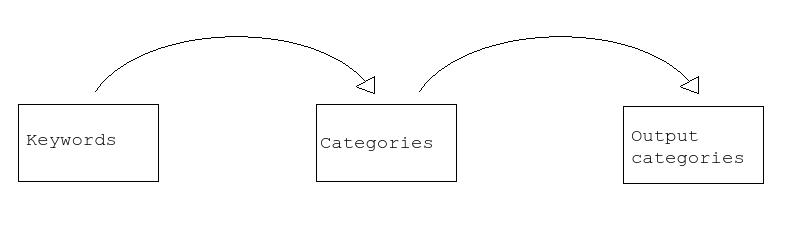
\includegraphics[width=1\textwidth]{classification_process.jpeg}
\caption{The classification process}
\label{fig:classification_process}
\end{figure}
%This classifier will be used as part of an automatic categorization process. 
%Our overall goal is therefore to make an automatic categorization that have a predefined keyword list and start by creating a mapping from each keyword to a category from another predefined list. Where the category of a text can be defined from the keywords found in the text. 